% 原书第 60—71 页：1.6、附录 1.A、1.B、习题；原第 72 页仅为出版商标志与网址页。
% 本文件不设章计数，不含 chapter 命令；所有公式按原印刷编号显式标注。
\FloatBarrier
\section{模拟与真实数据分析}
\label{sec:omics-simulation-real-data}

\subsection{用于模型评价的模拟研究}

可以通过大规模模拟研究，评价稀疏结构方程模型在基因型—表型网络分析中的表现（Wang et al. 2016）。这里考虑两类模拟：以 SNP 为单位的模拟和以基因为单位的模拟。模拟分别考察常见变异（$\mathrm{MAF}\leq 5\%$）、罕见变异（$\mathrm{MAF}<5\%$），以及常见变异与罕见变异各占一半的情形。基因型数据选自美国国家心肺血液研究所（NHLBI）的外显子测序计划（Exome Sequencing Project，ESP），包含 3248 名欧洲血统个体；随后利用这些数据生成一个包含 1,000,000 名个体的群体。

先介绍以 SNP 为单位的模拟。基因型—表型网络由两部分构成。第一部分是用有向无环图建模的表型网络；第二部分是基因型与表型之间的连接，其中箭头由基因型指向表型。我们随机生成一个基因型—表型网络结构，平均每个表型节点与另外三个表型节点相连。在用于表型子网络建模的结构方程模型中，若存在由节点 $j$ 指向节点 $i$ 的边，则从区间 $(0.5,1)$ 或 $(-1,-0.5)$ 上的均匀分布生成参数 $\Gamma_{ij}$；否则，令 $\Gamma_{ij}=0$。类似地，对于由基因型（SNP）节点 $j$ 指向表型节点 $i$ 的方向，若网络中存在这条边，则从区间 $(0,1)$ 或 $(-1,0)$ 上的均匀分布生成参数 $B_{ij}$；否则，令 $B_{ij}=0$。SNP 用其次要等位基因的数目编码。利用随机生成的网络结构及结构方程中的参数，我们根据模型
\[
Y=-XB\Gamma^{-1}+\varepsilon\Gamma^{-1}
\]
生成表型，其中 $\varepsilon\sim N(0,0.01\times I)$，$I$ 为单位矩阵，$X$ 为基因型编码指示变量构成的矩阵。在随机生成的表型网络中，每个节点的期望度数为 3。模拟重复 100 次。我们采用五折交叉验证确定惩罚参数 $\lambda$，再将其用于稀疏结构方程模型的计算。

采用检出功效（power of detection，PD）和错误发现率（FDR）两项指标，评价算法识别网络结构的表现。具体地，令 $N_t$ 为 1000 次网络重复中边的总数，$\widehat N_t$ 为推断算法检测到的边的总数；$N_{\mathrm{true}}$ 为模拟网络中检测到的真实边总数，$N_{\mathrm{false}}$ 为 $\widehat N_t$ 中检测到的错误边总数。于是，检出功效定义为 $N_{\mathrm{True}}/N_t$，错误发现率定义为 $N_{\mathrm{False}}/\widehat N_t$。

在以 SNP 为单位的模拟中，我们首先比较采用 ADMM 算法的稀疏两阶段结构方程模型（sparse two-stage SEM，S2SEM）与采用坐标上升算法的稀疏极大似然结构方程模型（sparse maximum likelihood SEM，SML）（Cai et al. 2013）。SML 方法假定每个表型都有一个先验已知的数量性状基因座（quantitative trait locus，QTL），并且只推断表型网络。因此，在这项比较中，我们只计算表型网络的检出功效和错误发现率。

首先假定每个 QTL 只与一个表型相连，不存在多效性效应，比较 S2SEM 与 SML 的功效及错误发现率。我们考虑两种情形：10 个表型和 10 个 SNP，以及 30 个表型和 30 个 SNP；并分别考察常见变异、罕见变异和全部变异这三类 SNP。结果见图 1.16。我们观察到，当变异均为常见变异时，SML 的功效高于 S2SEM，错误发现率也更低。但是，一旦纳入罕见变异，SML 的功效便显著下降，错误发现率随之升高，S2SEM 的表现则明显优于 SML。在假定存在遗传多效性的情形下，两种方法的功效和错误发现率也呈现类似结果。

% 原始嵌入曲线位图，原图位置上的中文标签由 TikZ 排印。
\begin{figure}[htbp]
\centering
\begin{tikzpicture}[x=0.08mm,y=-0.08mm,inner sep=0pt]
\node[anchor=north west] (ch01dfig16data) at (0,0) {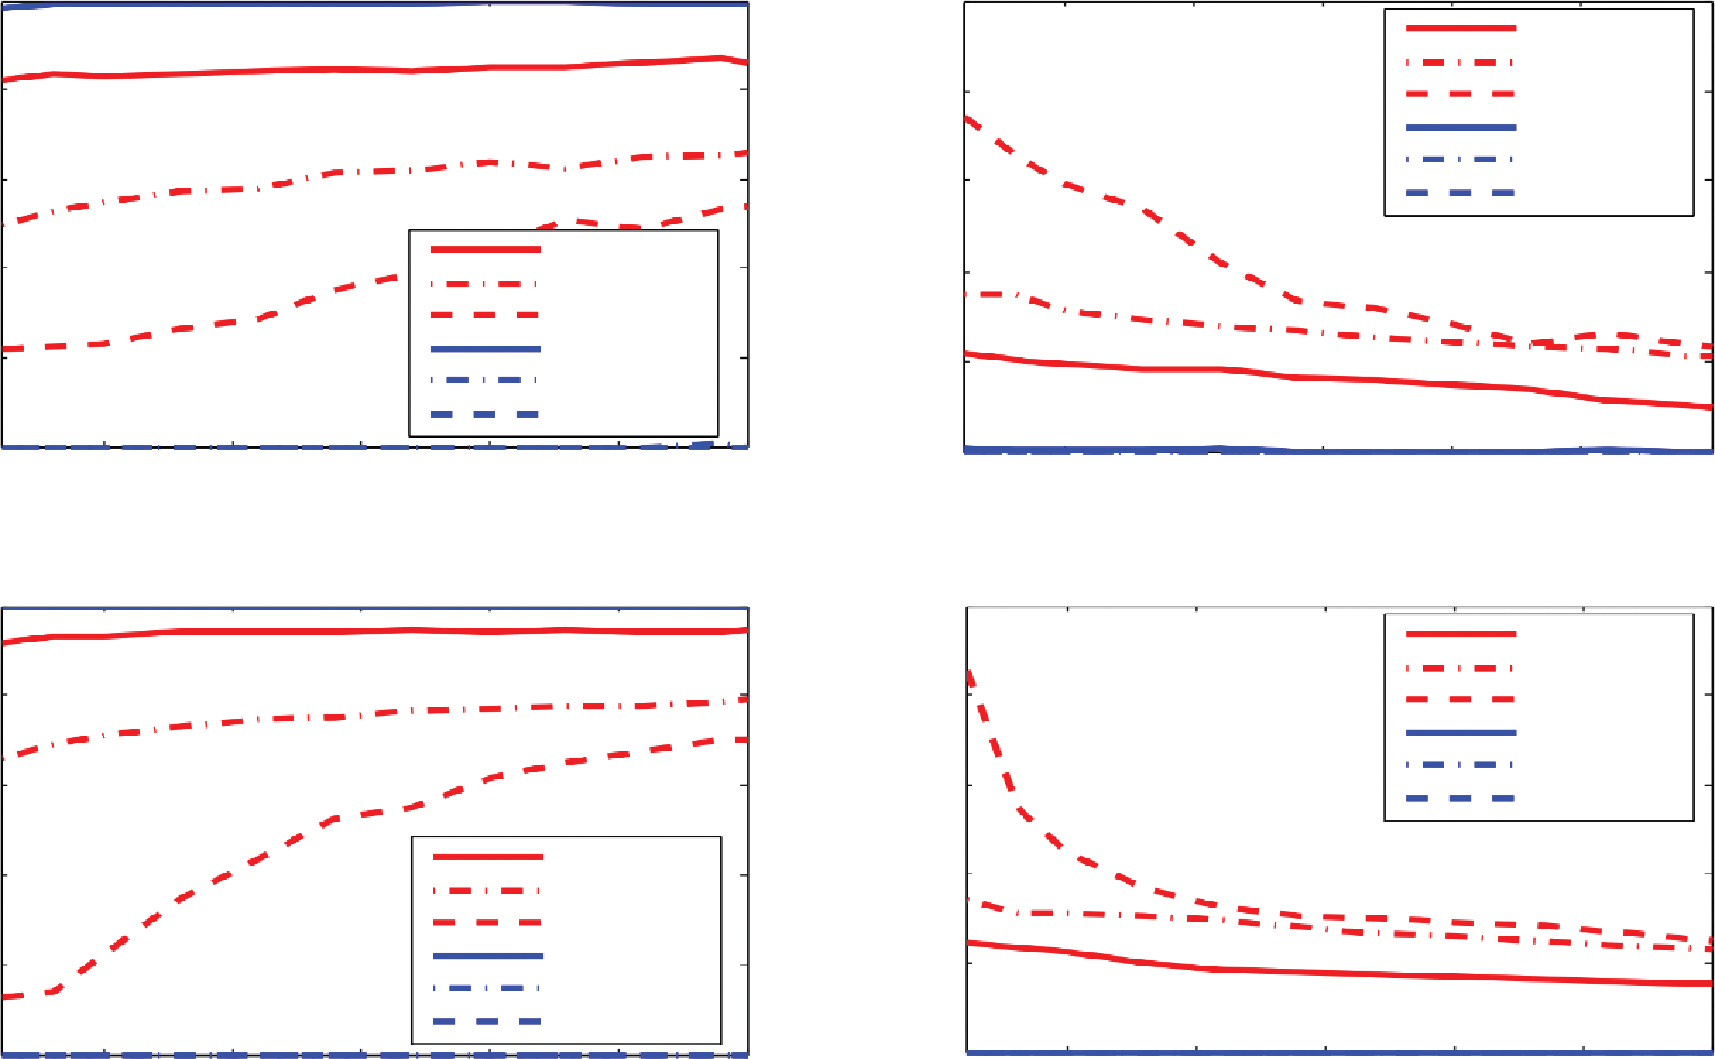
\includegraphics[width=137.2mm]{figures/ch01d_figure16_data.png}};
\node[font=\fontsize{7.0}{8}\selectfont] at (358.755,-29.070) {10 个表型，10 个 SNP：PD};
\node[font=\fontsize{7.0}{8}\selectfont] at (1324.962,-29.070) {10 个表型，10 个 SNP：FDR};
\node[font=\fontsize{7.0}{8}\selectfont] at (369.144,577.220) {30 个表型，30 个 SNP：PD};
\node[font=\fontsize{7.0}{8}\selectfont] at (1327.419,577.220) {30 个表型，30 个 SNP：FDR};
\node[rotate=90,font=\fontsize{7.0}{8}\selectfont] at (-75.867,224.994) {检出功效};
\node[rotate=90,font=\fontsize{7.0}{8}\selectfont] at (-75.867,832.723) {检出功效};
\node[font=\fontsize{7.0}{8}\selectfont] at (366.742,516.359) {样本量};
\node[font=\fontsize{7.0}{8}\selectfont] at (356.153,1119.854) {样本量};
\node[font=\fontsize{7.0}{8}\selectfont] at (1361.018,1119.854) {样本量};
\node[rotate=90,font=\fontsize{7.0}{8}\selectfont] at (889.461,840.340) {错误发现率};
\node[rotate=90,font=\fontsize{7.0}{8}\selectfont] at (889.461,234.179) {错误发现率};
\node[font=\fontsize{7.0}{8}\selectfont] at (-14.128,5.069) {1};
\node[font=\fontsize{7.0}{8}\selectfont] at (-26.496,94.094) {0.8};
\node[font=\fontsize{7.0}{8}\selectfont] at (-26.496,183.111) {0.6};
\node[font=\fontsize{7.0}{8}\selectfont] at (-26.496,272.135) {0.4};
\node[font=\fontsize{7.0}{8}\selectfont] at (-26.496,361.152) {0.2};
\node[font=\fontsize{7.0}{8}\selectfont] at (-14.128,450.177) {0};
\node[font=\fontsize{7.0}{8}\selectfont] at (945.553,5.069) {1};
\node[font=\fontsize{7.0}{8}\selectfont] at (933.185,94.093) {0.8};
\node[font=\fontsize{7.0}{8}\selectfont] at (933.185,183.111) {0.6};
\node[font=\fontsize{7.0}{8}\selectfont] at (933.185,272.135) {0.4};
\node[font=\fontsize{7.0}{8}\selectfont] at (933.185,361.152) {0.2};
\node[font=\fontsize{7.0}{8}\selectfont] at (945.553,454.412) {0};
\node[font=\fontsize{7.0}{8}\selectfont] at (949.789,610.685) {1};
\node[font=\fontsize{7.0}{8}\selectfont] at (937.420,699.706) {0.8};
\node[font=\fontsize{7.0}{8}\selectfont] at (937.420,788.727) {0.6};
\node[font=\fontsize{7.0}{8}\selectfont] at (937.420,877.747) {0.4};
\node[font=\fontsize{7.0}{8}\selectfont] at (937.420,966.768) {0.2};
\node[font=\fontsize{7.0}{8}\selectfont] at (949.789,1055.789) {0};
\node[font=\fontsize{7.0}{8}\selectfont] at (-15.534,610.685) {1};
\node[font=\fontsize{7.0}{8}\selectfont] at (-27.903,699.706) {0.8};
\node[font=\fontsize{7.0}{8}\selectfont] at (-27.903,788.726) {0.6};
\node[font=\fontsize{7.0}{8}\selectfont] at (-27.903,877.747) {0.4};
\node[font=\fontsize{7.0}{8}\selectfont] at (-27.903,966.768) {0.2};
\node[font=\fontsize{7.0}{8}\selectfont] at (-15.534,1055.789) {0};
\node[font=\fontsize{7.0}{8}\selectfont] at (1067.584,1081.927) {500};
\node[font=\fontsize{7.0}{8}\selectfont] at (1195.839,1081.927) {1000};
\node[font=\fontsize{7.0}{8}\selectfont] at (1324.092,1081.927) {1500};
\node[font=\fontsize{7.0}{8}\selectfont] at (1452.344,1081.927) {2000};
\node[font=\fontsize{7.0}{8}\selectfont] at (1580.603,1081.927) {2500};
\node[font=\fontsize{7.0}{8}\selectfont] at (1708.855,1081.927) {3000};
\node[font=\fontsize{7.0}{8}\selectfont] at (1361.017,516.362) {样本量};
\node[font=\fontsize{7.0}{8}\selectfont] at (1067.584,474.197) {500};
\node[font=\fontsize{7.0}{8}\selectfont] at (1195.839,474.197) {1000};
\node[font=\fontsize{7.0}{8}\selectfont] at (1324.092,474.197) {1500};
\node[font=\fontsize{7.0}{8}\selectfont] at (1452.344,474.197) {2000};
\node[font=\fontsize{7.0}{8}\selectfont] at (1580.603,474.197) {2500};
\node[font=\fontsize{7.0}{8}\selectfont] at (1708.855,474.197) {3000};
\node[font=\fontsize{7.0}{8}\selectfont] at (102.955,474.197) {500};
\node[font=\fontsize{7.0}{8}\selectfont] at (231.211,474.197) {1000};
\node[font=\fontsize{7.0}{8}\selectfont] at (359.466,474.197) {1500};
\node[font=\fontsize{7.0}{8}\selectfont] at (487.718,474.197) {2000};
\node[font=\fontsize{7.0}{8}\selectfont] at (615.970,474.197) {2500};
\node[font=\fontsize{7.0}{8}\selectfont] at (744.240,474.197) {3000};
\node[font=\fontsize{7.0}{8}\selectfont] at (102.955,1081.927) {500};
\node[font=\fontsize{7.0}{8}\selectfont] at (231.211,1081.927) {1000};
\node[font=\fontsize{7.0}{8}\selectfont] at (359.466,1081.927) {1500};
\node[font=\fontsize{7.0}{8}\selectfont] at (487.718,1081.927) {2000};
\node[font=\fontsize{7.0}{8}\selectfont] at (615.970,1081.927) {2500};
\node[font=\fontsize{7.0}{8}\selectfont] at (744.240,1081.927) {3000};
\node[anchor=west,font=\fontsize{5.6}{8}\selectfont] at (556.186,252.391) {S2SEM-常见};
\node[anchor=west,font=\fontsize{5.6}{8}\selectfont] at (556.186,285.648) {S2SEM-全部};
\node[anchor=west,font=\fontsize{5.6}{8}\selectfont] at (556.186,320.417) {S2SEM-罕见};
\node[anchor=west,font=\fontsize{5.6}{8}\selectfont] at (556.186,353.974) {SML-常见};
\node[anchor=west,font=\fontsize{5.6}{8}\selectfont] at (556.186,389.200) {SML-全部};
\node[anchor=west,font=\fontsize{5.6}{8}\selectfont] at (556.186,420.645) {SML-罕见};
\node[anchor=west,font=\fontsize{5.6}{8}\selectfont] at (556.186,856.592) {S2SEM-常见};
\node[anchor=west,font=\fontsize{5.6}{8}\selectfont] at (556.186,889.849) {S2SEM-全部};
\node[anchor=west,font=\fontsize{5.6}{8}\selectfont] at (556.186,924.618) {S2SEM-罕见};
\node[anchor=west,font=\fontsize{5.6}{8}\selectfont] at (556.186,958.173) {SML-常见};
\node[anchor=west,font=\fontsize{5.6}{8}\selectfont] at (556.186,993.399) {SML-全部};
\node[anchor=west,font=\fontsize{5.6}{8}\selectfont] at (556.186,1024.844) {SML-罕见};
\node[anchor=west,font=\fontsize{5.6}{8}\selectfont] at (1529.233,634.656) {S2SEM-常见};
\node[anchor=west,font=\fontsize{5.6}{8}\selectfont] at (1529.233,667.913) {S2SEM-全部};
\node[anchor=west,font=\fontsize{5.6}{8}\selectfont] at (1529.233,702.682) {S2SEM-罕见};
\node[anchor=west,font=\fontsize{5.6}{8}\selectfont] at (1529.233,736.242) {SML-常见};
\node[anchor=west,font=\fontsize{5.6}{8}\selectfont] at (1529.233,771.468) {SML-全部};
\node[anchor=west,font=\fontsize{5.6}{8}\selectfont] at (1529.233,802.913) {SML-罕见};
\node[anchor=west,font=\fontsize{5.6}{8}\selectfont] at (1532.054,29.042) {S2SEM-常见};
\node[anchor=west,font=\fontsize{5.6}{8}\selectfont] at (1532.054,62.299) {S2SEM-全部};
\node[anchor=west,font=\fontsize{5.6}{8}\selectfont] at (1532.054,97.068) {S2SEM-罕见};
\node[anchor=west,font=\fontsize{5.6}{8}\selectfont] at (1532.054,130.625) {SML-常见};
\node[anchor=west,font=\fontsize{5.6}{8}\selectfont] at (1532.054,165.849) {SML-全部};
\node[anchor=west,font=\fontsize{5.6}{8}\selectfont] at (1532.054,197.294) {SML-罕见};
\node[font=\fontsize{7.0}{8}\selectfont] at (-90.501,1165.288) {(c)};
\node[font=\fontsize{7.0}{8}\selectfont] at (-93.771,529.356) {(a)};
\node[font=\fontsize{7.0}{8}\selectfont] at (873.091,529.356) {(b)};
\node[font=\fontsize{7.0}{8}\selectfont] at (872.645,1163.174) {(d)};
\end{tikzpicture}
\origfig{16}{S2SEM 与 SML 推断表型网络的表现。分别在表型和基因型数目均为 10〔(a)、(b)〕及均为 30〔(c)、(d)〕时，比较两种方法的检出功效与错误发现率。图中“常见”“罕见”“全部”分别对应原图的 Com、Rare、All。}
\label{fig:omics-s2sem-sml}
\end{figure}


与 SML 相比，S2SEM 推断网络所需的计算时间少得多，而且可以构建基因型—表型网络。已有研究报告，在包含 100 个表型和 1000 个 SNP 的基因型—表型网络中，无论考察常见变异、罕见变异，还是同时考察两者，S2SEM 随样本量变化的网络结构检出功效仍然较高，错误发现率则较低（Wang et al. 2016）。

以基因组区域或基因为分析单位的函数型结构方程模型（FSEM），能够降低数据维数并提高网络分析的功效。在常见变异、罕见变异和同时包含常见与罕见变异这三种情形下，以基因为单位的 FSEM 都比以 SNP 为单位的结构方程模型具有高得多的功效和更低的错误发现率。值得关注的是，即使只考察罕见变异，当样本量超过 3000 时，以基因为单位的方法也能达到高达 85\% 的功效（Wang et al. 2016）。

\FloatBarrier
\subsection{真实数据实例中的应用}

为说明方法的表现，研究者将以基因为分析单位的稀疏函数型结构方程模型，应用于包含 765 名个体的 UK-10K 数据集样本，以及包含 21,501 名个体的中国泰州队列研究数据集。两个数据集共有的 13 个表型汇总于表 1.1。我们使用稀疏结构方程模型，分别从两个数据集构建表型网络。对于每个数据集，都识别出一个含有 13 个节点和 54 条边的表型网络（Wang，2016）。由 UK-10K 数据和泰州数据得到的两个表型网络共有 33 条边，重复验证率为 61\%。这表明，结构方程模型推断网络的方法具有稳健性。

\begin{table}[htbp]
\centering
\origtable{1}{UK-10K 与泰州队列共有的 13 个表型。}
\label{tab:omics-common-phenotypes}
\small
\setlength{\tabcolsep}{4pt}
\begin{tabularx}{\textwidth}{@{}>{\raggedright\arraybackslash}Xrrr@{\hspace{1.2em}}rrr@{}}
\toprule
 & \multicolumn{3}{c}{TWINSUK，756 例} & \multicolumn{3}{c}{泰州，21,501 例} \\
\cmidrule(lr){2-4}\cmidrule(l){5-7}
表型 & 均值 & 中位数 & 标准差 & 均值 & 中位数 & 标准差 \\
\midrule
血糖（mmol/l） & 5.04 & 4.90 & 0.86 & 5.43 & 5.16 & 1.55 \\
总胆固醇（mmol/l） & 5.55 & 5.50 & 1.03 & 5.01 & 4.94 & 1.04 \\
HDL（mmol/l） & 1.85 & 1.81 & 0.48 & 1.51 & 1.46 & 1.11 \\
LDL（mmol/l） & 3.17 & 3.09 & 0.99 & 2.41 & 2.49 & 0.84 \\
甘油三酯（mmol/l） & 1.16 & 0.99 & 0.64 & 1.68 & 1.22 & 1.79 \\
肌酐（umol/l） & 75.63 & 74.00 & 30.20 & 68.74 & 64.80 & 26.99 \\
尿素（mmol/l） & 5.02 & 4.80 & 1.43 & 6.02 & 5.80 & 2.48 \\
胆红素（umol/l） & 8.94 & 8.00 & 3.51 & 14.11 & 13.40 & 5.86 \\
BMI（Kg/m$^2$） & 26.50 & 25.81 & 4.72 & 24.56 & 24.35 & 3.18 \\
WHR & 0.79 & 0.78 & 0.05 & 0.87 & 0.87 & 0.07 \\
心电图心率（次/min） & 66.58 & 66.00 & 10.29 & 76.75 & 76.00 & 10.61 \\
收缩压（mm/Hg） & 130.17 & 129.00 & 16.88 & 136.04 & 134.50 & 20.00 \\
舒张压（mm/Hg） & 78.55 & 78.00 & 9.77 & 81.51 & 81.00 & 12.27 \\
\bottomrule
\end{tabularx}
\end{table}

两个表型网络见图 1.17。其中，绿色边表示两个网络共有的边，粉红色边表示仅存在于 UK-10K 数据所构建网络中的边，黑色边表示仅存在于泰州队列数据所构建网络中的边，而原文所称的“pepper”色边表示两个网络中方向不同的同一条边。从图 1.17 可以看出，大多数估计得到的边有两个方向，只有少数边具有单一方向。如何将同时包含有向边与无向边的混合表型网络转化为有向图，将在第 2 章讨论。

% 原始嵌入网络图完整保留全部节点、边和箭头；中文节点标签由 TikZ 排印。
\begin{figure}[htbp]
\centering
\begin{tikzpicture}[x=0.1044mm,y=-0.1044mm,inner sep=0pt]
\node[anchor=north west] (ch01dfig17data) at (0,0) {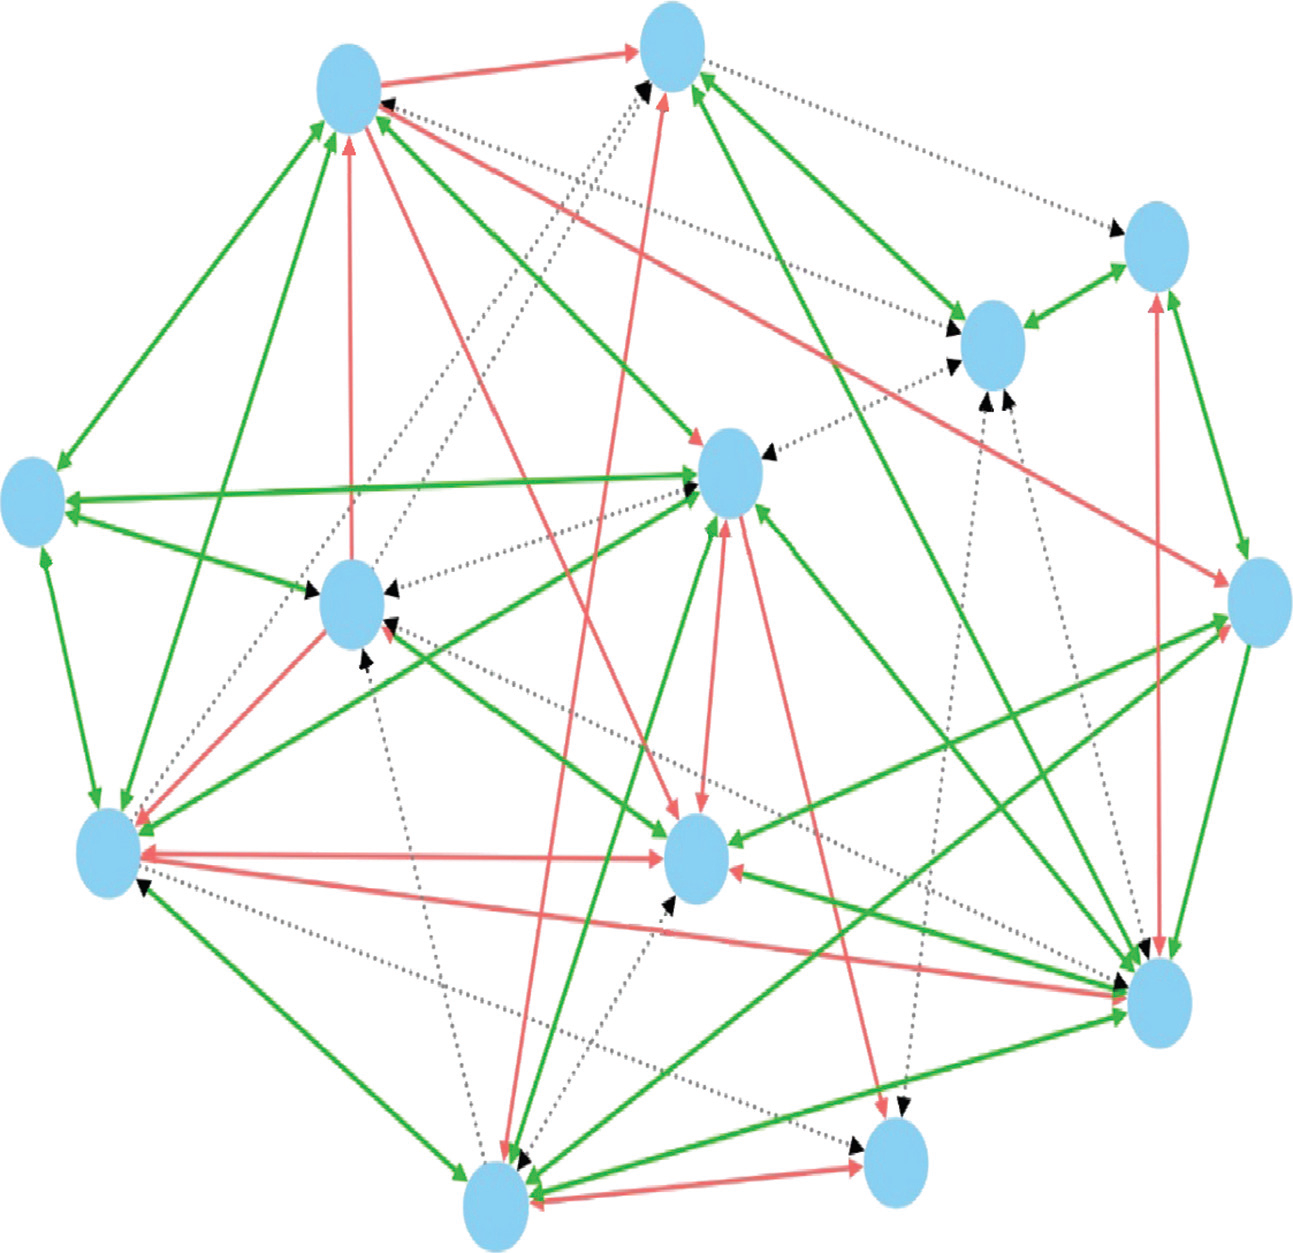
\includegraphics[width=135mm]{figures/ch01d_figure17_data.png}};
\node[fill=white,inner sep=0.5pt,font=\fontsize{8}{9}\selectfont] at (1162.487,1070.911) {WHR};
\node[fill=white,inner sep=0.5pt,font=\fontsize{8}{9}\selectfont] at (1286.196,669.837) {舒张压};
\node[fill=white,inner sep=0.5pt,font=\fontsize{8}{9}\selectfont] at (896.109,1229.734) {胆红素};
\node[fill=white,inner sep=0.5pt,font=\fontsize{8}{9}\selectfont] at (493.433,1274.677) {BMI};
\node[fill=white,inner sep=0.5pt,font=\fontsize{8}{9}\selectfont] at (106.990,925.282) {HDL};
\node[fill=white,inner sep=0.5pt,font=\fontsize{8}{9}\selectfont] at (717.845,927.522) {收缩压};
\node[fill=white,inner sep=0.5pt,font=\fontsize{8}{9}\selectfont] at (336.837,673.622) {血糖};
\node[fill=white,inner sep=0.5pt,font=\fontsize{8}{9}\selectfont] at (65.049,571.385) {总胆固醇};
\node[fill=white,inner sep=0.5pt,font=\fontsize{8}{9}\selectfont] at (741.064,541.052) {甘油三酯};
\node[fill=white,inner sep=0.5pt,font=\fontsize{8}{9}\selectfont] at (1016.175,418.600) {肌酐};
\node[fill=white,inner sep=0.5pt,font=\fontsize{8}{9}\selectfont] at (676.753,120.881) {尿素};
\node[fill=white,inner sep=0.5pt,font=\fontsize{8}{9}\selectfont] at (357.418,162.446) {LDL};
\node[fill=white,inner sep=0.5pt,font=\fontsize{8}{9}\selectfont] at (1184.078,312.995) {心率};
\end{tikzpicture}
\origfig{17}{从 UK-10K 和泰州队列数据集中识别出的两个表型网络，均包含 13 个节点和 54 条边。}
\label{fig:omics-real-phenotype-networks}
\end{figure}

\FloatBarrier
\section*{附录 1.A}
\addcontentsline{toc}{section}{附录 1.A}
\markright{附录 1.A}

考虑 $p$ 个基因。我们可以用一个汇总统计量，表示整个基因所包含的基因组信息。例如，对于第 $i$ 个基因，可以用 $y_i=\frac{1}{T_i}\int_{T_i}g_i(t)\,dt$ 汇总其基因组信息，其中 $g_i(t)$ 为基因型函数，$T_i$ 为第 $i$ 个基因所在的基因组区域；也可以使用前文定义的函数主成分得分。一般而言，这些汇总统计量渐近服从正态分布。因此，我们假定向量 $Y=[y_1,\ldots,y_p]^T$ 服从均值为零、协方差矩阵为 $\Sigma=(\sigma_{ij})$ 的正态分布。将浓度矩阵记为 $\Omega=(\sigma^{ij})=\Sigma^{-1}$。令 $y_{-(i,j)}$ 为从 $y$ 中去除变量 $y_i$ 和 $y_j$ 后，其余所有元素构成的随机向量。变量 $y_i$ 与 $y_j$ 的偏相关（partial correlation），定义为给定图中其余变量后两者的条件相关，即 $\rho^{ij}=\mathrm{Corr}(y_i,y_j\mid y_{-(i,j)})$。图的结构由浓度矩阵决定。变量 $y_i$ 与 $y_j$ 之间没有边，等价于浓度矩阵中的元素 $\sigma^{ij}=0$。

\Needspace{6\baselineskip}
理论上，有如下定理。

\begin{booktheorem}{1.A.1}
变量 $y_i$ 与 $y_j$ 之间没有边，当且仅当给定其余所有变量后，$y_i$ 与 $y_j$ 条件独立；这又等价于偏相关 $\rho^{ij}=0$。
\end{booktheorem}

\begin{bookproof}
将协方差矩阵分块为
\[
\Sigma=
\begin{bmatrix}
\Sigma_{(ij)} & \Sigma_{(ij,-ij)} \\
\Sigma_{(ij,-ij)} & \Sigma_{(-ij)}
\end{bmatrix},
\]
并令
\[
\begin{aligned}
\Sigma_{ij\cdot(-ij)}
&=\begin{bmatrix}
\sigma_{ii\cdot(-ij)} & \sigma_{ij\cdot(-ij)} \\
\sigma_{ji\cdot(-ij)} & \sigma_{jj\cdot(-ij)}
\end{bmatrix} \\
&=\Sigma_{ij}-\Sigma_{(ij,-ij)}\Sigma^{-1}_{(-jj)}\Sigma_{(ij,-ij)}.
\end{aligned}
\]
定理 1.4 表明，$\sigma^{ij}=0$ 当且仅当给定其余所有变量后，$y_i$ 与 $y_j$ 条件独立，而这又等价于 $\sigma_{(ij)\cdot(-ij)}=0$。首先建立 $\Sigma^{-1}$ 与 $\Sigma_{ij\cdot(-ij)}$ 之间的关系。定义
\[
\begin{aligned}
E_1&=\begin{bmatrix}I&0\\0&\Sigma^{-1}_{(-ij)}\end{bmatrix},
&E_2&=\begin{bmatrix}I&-\Sigma_{(ij,-ij)}\\0&I\end{bmatrix}, \\[3pt]
E_3&=\begin{bmatrix}\Sigma^{-1}_{ij\cdot(-ij)}&0\\0&I\end{bmatrix},
&E_4&=\begin{bmatrix}I&0\\-\Sigma^{-1}_{(-ij)}\Sigma_{(ij,-ij)}&I\end{bmatrix}.
\end{aligned}
\]
则有 $E_4E_3E_2E_1\Sigma=I$。因此，
\[
\Sigma^{-1}=\begin{bmatrix}\Sigma^{-1}_{ij\cdot(-ij)}&*\\ *&*\end{bmatrix}.
\]
由逆矩阵的定义，得到
\begin{equation}
\Sigma^{-1}_{ij(-ij)}=
\frac{1}{\Delta}
\begin{bmatrix}
\sigma_{jj(-ij)} & -\sigma_{ij(-ij)} \\
-\sigma_{ji(-ij)} & \sigma_{ii(-ij)}
\end{bmatrix},
\tag{1.A.1}
\end{equation}
其中 $\Delta=\sigma_{ii\cdot(-ij)}\sigma_{jj\cdot(-ij)}-\sigma_{ij\cdot(-ij)}\sigma_{ji\cdot(-ij)}$。这意味着
\begin{equation}
\sigma^{ij}=\frac{-\sigma_{ij(-ij)}}{\Delta}.
\tag{1.A.2}
\end{equation}
式 (1.A.2) 表明，$\sigma^{ij}=0$ 当且仅当 $\sigma_{ij\cdot(-ij)}=0$。因此，当图中变量的联合分布为正态分布时，这意味着给定其余所有变量后，$y_i$ 与 $y_j$ 条件独立。接下来证明，它又等价于 $\rho^{ij}=0$。

事实上，由定义，$\rho^{ij}=\sigma_{ij\cdot(-ij)}/\sqrt{\sigma_{ii\cdot(-ij)}\sigma_{jj\cdot(-ij)}}$。由式 (1.A.1) 可得
\begin{equation}
\sigma^{ii}=\frac{\sigma_{jj(-ij)}}{\Delta},\qquad
\sigma^{jj}=\frac{\sigma_{ii(-ij)}}{\Delta}.
\tag{1.A.3}
\end{equation}
结合式 (1.A.2) 与式 (1.A.3)，得到
\begin{equation}
\rho^{ij}
=\frac{\sigma_{ij(-ij)}}{\sqrt{\sigma_{ii(-ij)}\sigma_{jj(-ij)}}}
=-\frac{\Delta\sigma^{ij}}{\sqrt{\Delta^2\sigma^{ii}\sigma^{jj}}}
=-\frac{\sigma^{ij}}{\sqrt{\sigma^{ii}\sigma^{jj}}},
\tag{1.A.4}
\end{equation}
这说明，$\rho^{ij}=0$ 当且仅当 $\sigma^{ij}=0$，也当且仅当给定其余所有变量后，$y_i$ 与 $y_j$ 条件独立。
\end{bookproof}

偏相关系数与多元回归系数密切相关，如定理 1.A.2 所示。

\begin{booktheorem}{1.A.2}
假定多元回归为 $y_i=\beta_{ij}y_j+\sum_{k\ne i,j}\beta_{ik}y_k+\varepsilon_i$，则有
\[
\beta_{ij}=\rho^{ij}\sqrt{\frac{\sigma^{jj}}{\sigma^{ii}}}.
\]
\end{booktheorem}

\begin{bookproof}
系数 $\beta_{ij}$ 是 $y_i$ 关于 $y_j$ 及 $y_k$（$k\ne i,j$）的多元回归方程中，$y_i$ 对 $y_j$ 的回归系数。因此，有
\[
\begin{aligned}
\beta_{ij}
&=\frac{\mathrm{cov}(y_i,y_j\mid Y_{(-ij)})}{\mathrm{var}(y_j\mid Y_{(-ij)})}
=\frac{\sigma_{ij(-ij)}}{\sigma_{jj(-ij)}} \\
&=\rho^{ij}\sqrt{\frac{\sigma_{ii(-ij)}}{\sigma_{jj(-ij)}}}
=\rho^{ij}\sqrt{\frac{\sigma^{jj}}{\sigma^{ii}}}.
\end{aligned}
\]
多元回归可以改写为
\begin{equation}
y_i=\beta_{ij(-ij)}y_j+\sum_{k\ne i,j}\beta_{ik(-ik)}y_k+\varepsilon_i.
\tag{1.A.5}
\end{equation}
考虑 $y_i$ 对 $y_j$ 的回归 $y_i=\beta_{ij}y_j+\varepsilon_i$，可知
\begin{equation}
\beta_{ij}y_j+\varepsilon_i
=\beta_{ij(-ij)}y_j+\sum_{k\ne i,j}\beta_{ik(-ik)}y_k+\varepsilon_i.
\tag{1.A.6}
\end{equation}
在式 (1.A.6) 两边分别与 $y_j$ 求协方差，得到
\begin{equation}
\beta_{ij}\sigma_{jj}
=\beta_{ij(-ij)}\sigma_{jj}+\sum_{k\ne i,j}\beta_{ik(-ik)}\sigma_{kj}.
\tag{1.A.7}
\end{equation}
式 (1.A.7) 两边同除以 $\sigma_{jj}$，得到
\begin{equation}
\beta_{ij}=\beta_{ij(-ij)}+\sum_{k\ne i,j}\beta_{ik(-ik)}\beta_{kj}.
\tag{1.A.8}
\end{equation}
\end{bookproof}

\FloatBarrier
\section*{附录 1.B}
\addcontentsline{toc}{section}{附录 1.B}
\markright{附录 1.B}

现在推导算法 1.2。首先考虑关于 $\Theta$ 的最小化。对拉格朗日函数 $L_\rho(\Theta^{(1)})$ 关于 $\Theta^{(1)}$ 求导，并令导数为零，得到
\begin{equation}
\begin{aligned}
\frac{\partial L_\rho}{\partial\Theta^{(1)}}
={}&n_1S^{(1)}-n_1\bigl(\Theta^{(1)}\bigr)^{(-1)} \\
&+\rho\bigl(\Theta^{(1)}-\Theta^{(2)}-(V+W)+U_1
+\Theta^{(1)}-Z^{(1)}+U_3\bigr)=0,
\end{aligned}
\tag{1.B.1}
\end{equation}
因此有
\begin{equation}
\begin{aligned}
\Theta^{(1)}-\frac{n_1}{2\rho}\bigl(\Theta^{(1)}\bigr)^{-1}
={}&\frac12\bigl(\Theta^{(2)}+V+W-U_1-U_3+Z^{(1)}\bigr) \\
&-\frac{n_1}{2\rho}S^{(1)}.
\end{aligned}
\tag{1.B.2}
\end{equation}
令
\[
B_1=\frac12\bigl(\Theta^{(2)}+V+W-U_1-U_3+Z^{(1)}\bigr)-\frac{n_1}{2\rho}S^{(1)}.
\]
为求解矩阵方程 (1.B.2)，我们对矩阵 $B_1$ 作正交特征值分解：
\begin{equation}
B_1=Q_1\Lambda_1Q_1^T,
\tag{1.B.3}
\end{equation}
其中 $\Lambda_1=\diag(\lambda_1^{(1)},\ldots,\lambda_p^{(1)})$，且 $QQ^T=Q^TQ=I$。

在式 (1.B.2) 左边乘以正交归一矩阵 $Q^T$，右边乘以 $Q$，得到
\begin{equation}
\widetilde X_1-\frac{n_1}{2\rho}\widetilde X_1^{-1}=\Lambda_1,
\tag{1.B.4}
\end{equation}
其中 $\widetilde X_1=Q_1^T\Theta^{(1)}Q_1$ 为对角矩阵。

因此，式 (1.B.4) 给出下列线性代数方程：
\begin{equation}
\widetilde X_{ii}-\frac{n_1}{2\rho\widetilde X_{ii}}=\lambda_i,
\qquad i=1,\ldots,p.
\tag{1.B.5}
\end{equation}
求解式 (1.B.5)，并取正根，得到
\[
\widetilde X_{ii}=\frac{\lambda_i+\sqrt{\lambda_i^2+\dfrac{2n_1}{\rho}}}{2},
\qquad i=1,\ldots,p.
\]
第一个子网络的精度矩阵估计为
\begin{equation}
\widehat\Theta^{(1)(l+1)}=Q_1\widetilde X_1Q_1^T,
\tag{1.B.6}
\end{equation}
其中 $\widetilde X_1=\diag(\widetilde X_{11},\ldots,\widetilde X_{pp})$。

类似地，对于 $\Theta^{(2)}$，有
\[
\begin{aligned}
\frac{\partial L_\rho}{\partial\Theta^{(2)}}
={}&n_2S^{(2)}-n_2\bigl(\Theta^{(2)}\bigr)^{-1} \\
&-\rho\Bigl[\Theta^{(1)(l+1)}-\Theta^{(2)}-\bigl(V^{(l)}+W^{(l)}\bigr)+U_1^{(l)}\Bigr] \\
&+\rho\bigl(\Theta^{(2)}-Z^{(2)(l)}+U_4^{(l)}\bigr)=0,
\end{aligned}
\]
这给出矩阵方程
\begin{equation}
\Theta^{(2)}-\frac{n_2}{2\rho}\bigl(\Theta^{(2)}\bigr)^{-1}=B_2,
\tag{1.B.7}
\end{equation}
其中
\[
\begin{aligned}
B_2={}&\frac12\Bigl[\Theta^{(1)(l+1)}-\bigl(V^{(l)}+W^{(l)}\bigr)+U_1^{(l)}
+Z^{(2)(l)}-U_4^{(l)}\Bigr] \\
&-\frac{n_2}{2\rho}S^{(2)}.
\end{aligned}
\]
对矩阵 $B_2$ 作正交特征值分解，得到
\begin{equation}
B_2=Q_2\Lambda_2Q_2^T.
\tag{1.B.8}
\end{equation}
结合式 (1.B.7) 与式 (1.B.8)，有
\begin{equation}
\widetilde X_2-\frac{n_2}{2\rho}\bigl(\widetilde X_2\bigr)^{-1}=\Lambda_2,
\tag{1.B.9}
\end{equation}
其中 $\widetilde X_2=Q_2^T\Theta^{(2)}Q_2$，$\Lambda_2=\diag(\lambda_i^{(2)},\ldots,\lambda_p^{(2)})$。

求解矩阵方程 (1.B.9)，得到
\[
\widetilde X_{ii}=\frac{\lambda_i^{(2)}+\sqrt{\bigl(\lambda_i^{(2)}\bigr)^2+\dfrac{2n_2}{\rho}}}{2},
\qquad \widetilde X_2=\diag(\widetilde X_{11},\ldots,\widetilde X_{pp}).
\]
因此有
\begin{equation}
\Theta^{(2)(l+1)}=Q_2\widetilde X_2Q_2^T.
\tag{1.B.10}
\end{equation}
令 $\partial L_\rho/\partial W=0$，得到
\begin{equation}
\begin{aligned}
W^{(l+1)}=\frac12\Bigl[{}&\Theta^{(1)(l+1)}-\Theta^{(2)(l+1)}+\bigl(V^{(l)}\bigr)^T \\
&-V^{(l)}+U_1^{(l)}+\bigl(U_2^{(l)}\bigr)^T\Bigr].
\end{aligned}
\tag{1.B.11}
\end{equation}

接下来用广义梯度（generalized gradient）或次梯度（subgradient），求出 $Z^{(1)}$、$Z^{(2)}$ 和 $V$。

对 $L_\rho$ 关于 $Z^{(1)}$ 求广义梯度，得到
\begin{equation}
\frac{\partial L_\rho}{\partial Z^{(1)}}
=\lambda_1\Gamma_1-\rho\bigl(\Theta^{(1)(l+1)}-Z^{(1)}+U_3^{(l)}\bigr)=0,
\tag{1.B.12}
\end{equation}
其中 $\Gamma_1=[\gamma_1,\ldots,\gamma_p]^T$，且
\[
\gamma_j=\begin{cases}
1,&Z_j^{(1)}>0,\\
[-1,1],&Z_j^{(1)}=0,\\
-1,&Z_j^{(1)}<0.
\end{cases}
\]
求解式 (1.B.12)，得到
\begin{equation}
Z^{(1)(l+1)}
=\sign\bigl(\Theta^{(1)(l+1)}+U_3^{(l)}\bigr)
\left(\left|\Theta^{(1)(l+1)}+U_3^{(l)}\right|-\frac{\lambda_1}{\rho}\right)_+.
\tag{1.B.13}
\end{equation}
类似地，有
\begin{equation}
Z^{(2)(l+1)}
=\sign\bigl(\Theta^{(2)(l+1)}+U_4^{(l)}\bigr)
\left(\left|\Theta^{(2)(l+1)}+U_4^{(l)}\right|-\frac{\lambda_1}{\rho}\right)_+.
\tag{1.B.14}
\end{equation}

现在考虑对 $V$ 施加组套索惩罚。对 $L_\rho$ 关于 $V_j$ 求广义梯度，得到
\begin{equation}
\begin{aligned}
\frac{\partial L_\rho}{\partial V_j}
={}&\lambda_2h-\rho\Bigl[\Theta^{(1)(l+1)}-\Theta^{(2)(l+1)}
-\bigl(V+W^{(l)}\bigr)+U_1^{(l)}\Bigr]_{(j)} \\
&+\rho\Bigl(V-\bigl(W^{(l+1)}\bigr)^T+U_2^{(l)}\Bigr)_{(j)}=0,
\end{aligned}
\tag{1.B.15}
\end{equation}
其中
\[
h=\begin{cases}
\dfrac{V_j}{\lVert V_j\rVert_2},&V_j\ne0,\\[6pt]
\lVert h\rVert_2<1,&V_j=0.
\end{cases}
\]
当 $V_j\ne0$ 时，经过代数运算，式 (1.B.15) 可化为
\begin{equation}
\left[1+\frac{\lambda_2}{2\rho\lVert V_j\rVert_2}\right]V_j=G_j,
\tag{1.B.16}
\end{equation}
其中
\[
\begin{aligned}
G_j=\frac12\Bigl[{}&\Theta^{(1)(l+1)}-\Theta^{(2)(l+1)}-W^{(l+1)}+U_1^{(l)} \\
&+\bigl(W^{(l+1)}\bigr)^T-U_2^{(l)}\Bigr].
\end{aligned}
\]
在式 (1.B.16) 两边取范数 $\lVert\cdot\rVert_2$，得到
\begin{equation}
\left[1+\frac{\lambda_2}{2\rho\lVert V_j\rVert_2}\right]\lVert V_j\rVert_2
=\lVert G_j\rVert_2.
\tag{1.B.17}
\end{equation}
由式 (1.B.17) 解出 $\lVert V_j\rVert_2$，得到
\begin{equation}
\lVert V_j\rVert_2=\lVert G_j\rVert_2-\frac{\lambda_2}{2\rho}.
\tag{1.B.18}
\end{equation}
当 $V_j\ne0$ 时，将式 (1.B.18) 代入式 (1.B.16)，得到
\begin{equation}
V_j=\left(1-\frac{\lambda_2}{2\rho\lVert G_j\rVert_2}\right)G_j.
\tag{1.B.19}
\end{equation}
结合式 (1.B.19) 以及 $L_\rho$ 在 $V_j=0$ 处的次梯度定义，得到解
\begin{equation}
V_j=\left(1-\frac{\lambda_2}{2\rho\lVert G_j\rVert_2}\right)_+G_j,
\qquad j=1,\ldots,p.
\tag{1.B.20}
\end{equation}

\FloatBarrier
\section*{习题}
\addcontentsline{toc}{section}{习题}
\markright{习题}

\begin{enumerate}[label=\textbf{习题 \arabic*.},leftmargin=4.8em,align=left,itemsep=0.7em]
\item 设 $\Sigma_x$ 为 $X$ 的协方差矩阵。将标准化预测变量定义为 $Z=\Sigma_x^{-1/2}(X-E(X))$。证明 $\mathrm{var}(Z)=1$。

\item 证明
\[
\frac12\sum_{i=1}^N(Y_i-\mu)^T\Sigma_p^{-1}(Y_i-\mu)
=\frac N2\Tr(\Sigma_p^{-1}S).
\]

\item 设 $A$ 与 $B$ 为矩阵。证明
\[
\frac{\partial(\Tr(AB))}{\partial B}=A^T,
\qquad
\frac{\partial\log|A|}{\partial A}=A^{-T}.
\]

\item 假定 $K=2$，推导求解带约束 (1.32) 的问题 (1.39) 的 ADMM 算法。

\item 推导求解三阶段最小二乘估计问题 (1.102) 的 ADMM 算法。

\item 证明，偏相关系数 $\rho_{yx\cdot z}$ 为
\[
\rho_{yx\cdot z}
=\frac{\rho_{yx}-\rho_{yz}\rho_{xz}}
{\bigl[(1-\rho_{yz}^2)(1-\rho_{xz}^2)\bigr]^{1/2}}.
\]

\item 给定 $Z$ 后，定义 $Y$ 对 $X$ 的回归系数 $\beta_{yx\cdot z}$ 为
$\beta_{yx\cdot z}=\sigma_{yx\cdot z}/\sigma_{xx\cdot z}$。证明
\[
\beta_{yx\cdot z}
=\frac{\sqrt{\sigma_{yy}}}{\sqrt{\sigma_{xx}}}
\frac{\rho_{yx}-\rho_{yz}\rho_{zx}}{1-\rho_{xz}^2}.
\]

\item 在图 1.8b 中，用路径系数表示并计算回归系数 $\beta_{yz\cdot x}$。

\item 考察图 1.11b。给定 $A$、$D$ 和 $B$，判断 $C$ 与 $E$ 是否独立。

\item 考察图 1.13c。利用结论 1.4，估计路径系数 $a$。
\end{enumerate}
